
%(BEGIN_QUESTION)
% Copyright 2006, Tony R. Kuphaldt, released under the Creative Commons Attribution License (v 1.0)
% This means you may do almost anything with this work of mine, so long as you give me proper credit

Unlike linear functions, the graphs of nonlinear functions do not have constant {\it slopes}.  Take for instance this graph of a ``parabola'' of the form $y = x^2$:

$$\includegraphics[width=15.5cm]{i01515x01.eps}$$

It is difficult (but not impossible) to estimate the slope of a nonlinear function such as this at any given point, just by looking at the graph.  If I were to ask you to estimate the slope of this equation's graph at $x=2$, how would you do it?

\underbar{file i01515}
%(END_QUESTION)





%(BEGIN_ANSWER)

One way is to draw a line that just grazes the curve of the parabola at the coordinate (2,4) and estimate its slope:

$$\includegraphics[width=15.5cm]{i01515x02.eps}$$

%(END_ANSWER)





%(BEGIN_NOTES)

Incidentally, the {\it exact} slope of the parabola at (2,4) is 4.

%INDEX% Mathematics, calculus: slope of a parabola

%(END_NOTES)


